%; whizzy chapter
% -initex iniptex -latex platex -format platex -bibtex jbibtex -fmt fmt
% 以上 whizzytex を使用する場合の設定。

%     Kansai Debian Meeting resources
%     Copyright (C) 2007 Takaya Yamashita
%     Thank you for Tokyo Debian Meeting resources

%     This program is free software; you can redistribute it and/or modify
%     it under the terms of the GNU General Public License as published by
%     the Free Software Foundation; either version 2 of the License, or
%     (at your option) any later version.

%     This program is distributed in the hope that it will be useful,
%     but WITHOUT ANY WARRANTY; without even the implied warranty of
%     MERCHANTABILITY or FITNESS FOR A PARTICULAR PURPOSE.  See the
%     GNU General Public License for more details.

%     You should have received a copy of the GNU General Public License
%     along with this program; if not, write to the Free Software
%     Foundation, Inc., 51 Franklin St, Fifth Floor, Boston, MA  02110-1301 USA

%  preview (shell-command (concat "evince " (replace-regexp-in-string "tex$" "pdf"(buffer-file-name)) "&"))
% 画像ファイルを処理するためにはebbを利用してboundingboxを作成。
%(shell-command "cd image200708; ebb *.png")

%%ここからヘッダ開始。

\documentclass[mingoth,a4paper]{jsarticle}
\usepackage{kansaimonthlyreport}
\usepackage[dvips]{xy}


% 日付を定義する、毎月変わります。
\newcommand{\debmtgyear}{2012}
\newcommand{\debmtgdate}{26}
\newcommand{\debmtgmonth}{2}
\newcommand{\debmtgnumber}{56}

\begin{document}

\begin{titlepage}

% 毎月変更する部分、本文の末尾も修正することをわすれずに

 第\debmtgnumber{}回 関西 Debian 勉強会資料

\vspace{2cm}

\begin{center}
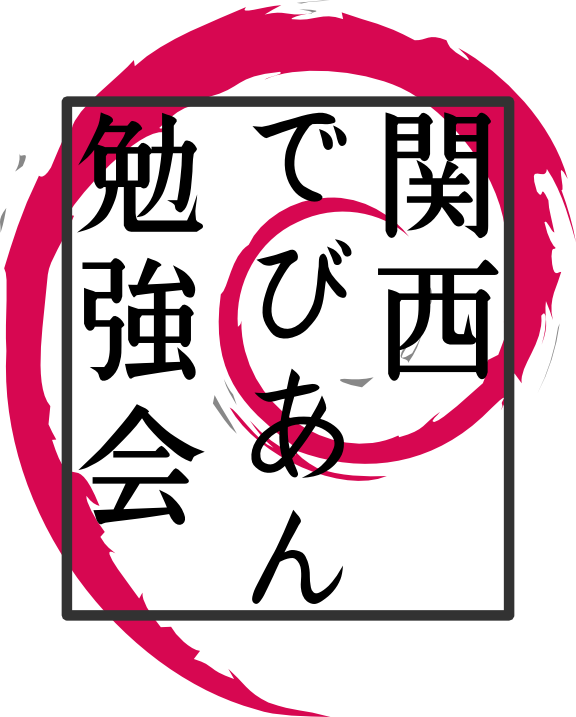
\includegraphics{image200802/kansaidebianlogo.png}
\end{center}

\begin{flushright}
\hfill{}関西 Debian 勉強会担当者 佐々木・倉敷・のがた・かわだ \\
\hfill{}\debmtgyear{}年\debmtgmonth{}月\debmtgdate{}日
\end{flushright}

\thispagestyle{empty}
\end{titlepage}

\dancersection{Introduction}{Debian JP}

 関西 Debian 勉強会はDebian GNU/Linux のさまざ
 まなトピック(新しいパッケージ、Debian 特有の機能の仕組、Debian 界隈で起
 こった出来事、などなど)について話し合う会です。

 目的として次の三つを考えています。
 \begin{itemize}
  \item MLや掲示板ではなく、直接顔を合わせる事での情報交換の促進
  \item 定期的に集まれる場所
  \item 資料の作成
 \end{itemize}

 それでは、楽しい一時をお楽しみ下さい。

\newpage

\begin{minipage}[b]{0.2\hsize}
 {\rotatebox{90}{\fontsize{80}{80}
{\gt 関西 Debian 勉強会}}}
\end{minipage}
\begin{minipage}[b]{0.8\hsize}
\hrule
\vspace{2mm}
\hrule
\setcounter{tocdepth}{1}
\tableofcontents
\vspace{2mm}
\hrule
\end{minipage}

\dancersection{最近のDebian関係のイベント報告}{Debian JP}

\subsection{第 55 回関西 Debian 勉強会}
55 回目の関西 Debian 勉強会は 1 月 28 日と 29 日の二日間の温泉合宿とし
て開催されました。\\
用意した apt のミラーサーバにソースパッケージが含まれていないという思わ
ぬ状況になりましたが、いつもの勉強会会場とは違った場所で集中して Hack
ができました。

\subsection{第 85 回東京エリア Debian 勉強会}
85 回目の東京エリア Debian 勉強会が 2 月 18 日に開催されました。\\
参加者が少なかったようですが KDE 開発、月刊 debhelper についての発表が
ありました。

\subsection{第 0 回福岡 Debian 勉強会}
同じく 2 月 18 日に福岡でも Debian 勉強会が開催されました。\\
0 回目となる今回の勉強会では Debian サーバの量産方法、DKMS とパッケージ
作成、キーサインパーティなどが行なわれたようです。\\
今後も Debian 勉強会が開催されていくとよいですね。

\clearpage

\dancersection{事前課題}{Debian JP}

今回は以下の課題を出題しました.
\begin{screen}
  \begin{description}
  \item[事前課題1] chroot について知っていますか。
    \begin{enumerate}
    \item 知らない人、chroot について調べたことを記入してください。
    \item 知っている人、PAM とオートマウンタの設定を触ったことはありますか?\\
      設定を触ったことがあるかたはその内容も記入してください。
    \end{enumerate}
  \item[事前課題2] DebianPolicy の7章に目を通しておいてください。
  \end{description}
\end{screen}

参加者の皆さんの解答は以下の通りです.

\begin{prework}{ kozo2 }
 \begin{enumerate}
  \item 知ってます
  \item ないです
  \item 読みます
 \end{enumerate}
\end{prework}

\begin{prework}{ 西山和広 }
\begin{enumerate}
 \item 知っています。
       \begin{itemize}
        \item PAM は pam-auth-update がなかった頃に libpam-ldap や libpam-tmpdir を使う設定をしました。オートマウンタは LDAP と組み合わせてホームディレクトリをマウントするのに使ったことがあります。
       \end{itemize}
\end{enumerate}
\end{prework}

\begin{prework}{ 佐藤誠 }
 \begin{enumerate}
  \item Yes. \\
        Linux From Scratch やGentoo Linux 
        のインストールのときに使っていました。

        Debian でもあれこれしたいときによく使います。

        最近はchrootが進化したような jail(8)とか
        lxc とかをちょこちょこ触っています
  \item ありません(汗
 \end{enumerate}
\end{prework}

\begin{prework}{ 川江 }
 \begin{enumerate}
  \item 同一PC上で、「異なる」root directory環境を提供する。
        \begin{itemize}
         \item 触った事はありません。
        \end{itemize}
  \item All right
 \end{enumerate}
\end{prework}

\begin{prework}{ 山下康成 }
 \begin{enumerate}
  \item 知ってます
        \begin{itemize}
         \item ずっと以前に触ったことはありますが、もう忘れてます。
        \end{itemize} 
  \item ざっと
 \end{enumerate}
\end{prework}

\begin{prework}{ 酒井 忠紀 }
 \begin{enumerate}
  \item chroot は、以下のように使用したことがあります。
        \begin{itemize}
         \item Debianベースにシステムにおいて、Linux Kernel を
               Android拡張し、chroot で Debian から Android に
               切り替える
         \item Andorid から Android の initプロセス配下を
               全て kill し、chroot 起動元の Debian のコンソールに戻る
        \end{itemize}
  \item PAM や オートマウンタ の設定を触ったことはありません。
        Debian の GNOME だと、USB などの自動マウントは
        autofs ではなく、nautilus で行っているのを
        見たことがあります。
 \end{enumerate}
\end{prework}

\begin{prework}{ かわだてつたろう }
 \begin{enumerate}
  \item 知っています。
        \begin{itemize}
         \item 触ったことはありません。発表を楽しみにしています。
        \end{itemize} 
  \item みておきます。
 \end{enumerate}
\end{prework}

\begin{prework}{ gdevmjc }
 \begin{enumerate}
  \item chroot について、知っています。\\
        PAM は、pam\_limits, pam\_chroot, pam\_ldap などの設定を触ったことがあります。pa\_wheel を追加したこともあります。
        オートマウンタは、マスターマップファイル、間接マップファイルともに触ったことが余す。 NFS や bind のマップを定義しました。
  \item はい、とりあえずチラ見しました。
 \end{enumerate}
\end{prework}

\begin{prework}{ 0xBCD1BC92 }

 \begin{enumerate}
  \item Yes 
        \begin{itemize}
         \item chrootで、PAMとオートマウンターの設定をしたことがない。 
        \end{itemize}
  \item Debian Policyの7章を眺めました。
 \end{enumerate}
\end{prework}

\begin{prework}{ 水野源 }
 \begin{enumerate}
  \item Yes
  \item autofsはYes、PAMは……忘れた
  \item ぉぅぃぇー
 \end{enumerate}
\end{prework}

\begin{prework}{ Y.YATSUO }
 \begin{enumerate}
  \item いいえ。 \\
        概要: \\
        ルートディレクトリを変更してプロセスがその外にアクセスできないようにする
       
        使われ方:
        \begin{itemize}
         \item Debian ではクリーンなビルド環境を作る
         \item セキュリティ強化の為にデーモン系をchroot環境で動かす 
        \end{itemize}
  \item 読んでおきます
 \end{enumerate}
\end{prework}

\begin{prework}{ lurdan }
 \begin{enumerate}
  \item yes
  \item no
  \item yes
 \end{enumerate}
\end{prework}

\begin{prework}{ のがたじゅん }
 \begin{enumerate}
  \item 知ってます。\\
        交野市のXubuntuの話の中で、LDAPで認証してホームをマウントするのにpam\_mountを使っただか使いたいとか話しがあって、その辺調べようと思ってたけどそのまま棚上げになってます。
  \item 日本語で読んでもいいですか (´;ω;`) \\
       \url{http://www.debian.or.jp/community/devel/debian-policy-ja/policy.ja.html/ch-relationships.html}
 \end{enumerate}
\end{prework}

\begin{prework}{ 佐々木洋平 }
 \begin{enumerate}
  \item 知ってます。git-buildpackage 用に cowbuilder を走らせる git-builder という shell script を使ってます。
  \item はい。某所ではサーバ御本尊の \$HOME を NFS でクライアントに提供していて、LDAP で認証後に autofs で mount しています。
  \item 読んでおきます。
 \end{enumerate}
\end{prework}

\clearpage
%% -*-tex-*-
%%
%% Copyright (C) 2012 Hiroshi Kubo  all rights reserved.
%% 本資料の著作権は、著者である久保博 <h-kubo@geisya.or.jp> にあります。
%%
%% This document material is licensed under the GNU General Public License version 2.0.
%% This document is originally in the form of LaTeX source code. This shall be referenced as the ``Corresponding Source''
%% Any compiled forms including DVI, Postscript, and PDF of the original source code shall be reference as the ``Object code''.
%% The complete license statement is appended at the tail of this file.
%% Also, license statement is mentioned in the last section of the document body.
%% 
%%
\dancersection{Autofs と pam\_chroot で作るマルチユーザー環境}{山城国の住人 \  久保博}
\subsection{はじめに}
皆さんの職場などの組織内では
ファイル共有サーバーやメール受信サーバーなど、組織内で情報を共有するためのサーバーを建てている場面もあるかと思いますが、
\begin{itemize}
\item 他のユーザーのホームディレクトリ内が覗けると不都合がある。
\item システム内の見せなくて良いファイルは見せたくない
\end{itemize}
など、運用面の制約があって、一般ユーザーにログインさせることを躊躇することはないですか?

そんな場合には、ユーザー毎に chroot 環境を用意できれば安心してログインさせられるようになります。
しかし、一般に知られた方法で実施しようとすると、ユーザー毎に chroot 先のシステム環境を用意することになりますし、
ユーザーを追加するたびに新しい chroot 環境を用意したりすれば、それだけ多くのディスクスペースも必要です。

ところが、 一工夫すると、一つの chroot 環境を複数のユーザー間で共用しながらユーザー間の chroot 環境は分離させることができるという、うまい話があるのです。

\subsection{道具立て}

そのための主な道具が autofs と pam\_chroot です。まずはそれぞれについて紹介をしておきましょう。

\subsubsection{pam\_chroot}

PAM とは Pluggable Authentication Modules の略\footnote{pam(5) の pam ではなく、 PAM(7) の PAM です。}です。
今はなき Sun Microsystems が世に出した認証処理の枠組で、動的ライブラリとしてモジュール化された処理、設定ファイル、呼出側へのAPI などから成ります。
pam\_chroot はその中で、認証処理の途中で認証されたユーザーセッションのプロセスを chroot 環境に放り込んでしまう処理を担当します。
次のコマンドでインストールしましょう。

\begin{verbatim}
$ sudo aptitude install libpam-chroot
\end{verbatim}

\subsubsection{Autofs}

Autofs は、オートマウンターと呼ばれるコマンドです。 
Sun Microsystems には NFS の拡張機能の automount というコマンドがあり、 NFS のボリュームのマウントをオンデマンドで行なってくれるデーモンでしたが、
Linux の autofs は NFS に限らず、他のファイルシステムもオンデマンドでマウントしてくれます。
次のコマンドでインストールしましょう。

\begin{verbatim}
$ sudo aptitude install autofs5
\end{verbatim}

\subsection{マルチユーザー環境の設計}
道具立てが揃ったら、次はどのように環境を構築をするか、考えます。
ログインしさえすればどんな場合でも chroot 環境に放り込んでしまうと、システム管理ができなくなりますから、
どんな条件でログインしたら chroot 環境に放り込むのか、そして、どういう機構を使って放り込むかを考えて決めてゆきます。

\subsubsection{アカウント}

「chroot させるユーザー」をどのように指定するか、まず問題になりますが、ユーザーのグループ設定を使うと後々設定が便利になりますので、お勧めします。
ここでは、chroot させるユーザーは staff グループに属することにします。
root と管理用アカウント(admin など)は、 staff グループに属させないように注意しましょう。

\subsubsection{ログインの経路}

次に、 ログイン処理のいずれかの段階でユーザーのプロセスを chroot 環境に放り込むわけですから、
どのようにログインするかを特定しておく必要があります。
いわば、システム内に足を踏み入れる玄関口を把握しておく、というわけです。
筆者の思いつく代表的な玄関口を挙げてみましょう。

\begin{itemize}
\item VGAコンソール
\item シリアルコンソール
\item ssh, sftp
\item rlogin, rcp, rsh
\item telnet
\item ftp
\item X セッションマネージャー (xdm, gdm,\ldots)
\item su, sudo
\end{itemize}

どうでしょう、読者のみなさんにとって、十分でしょうか。基本的には、これらの数だけ chroot の設定が必要です。

\subsubsection{chroot の処理を何に任せるか}

chroot する操作は、結局 chroot システムコールを呼び出す処理に帰着するわけですが、
ログインを司るアプリケーションサーバープログラムそのものが、 chroot に対応している場合もあります。
そうでない場合は、 PAM で認証の処理をする際に、 pam\_chroot で chroot するようにします。

設定さえすれば chroot させられるサーバーには、
\begin{itemize}
\item OpenSSH 4.8 以降
\item ProFTPD
\item vsftpd
\end{itemize}
がありますので、これらはサーバーの機能を活用し、他の経路でのログインでは pam\_chroot で chroot させることにします。

\subsection{設定}

\subsubsection{chroot の設定}

ここでは、{\tt /jail/chroot} の下にユーザー名と同じ名前のディレクトリを作り、
各ユーザーがログインしたら、そのディレクトリの下に chroot させるようにします。
例えば、ユーザー名 {\tt hiroshi} でログインしたら、 {\tt /jail/chroot/hiroshi } の下に chroot することになります。
まずは、chroot 先として必要なディレクトリを作ります。

\begin{verbatim}
mkdir /jail/chroot
\end{verbatim}


\subsubsubsection{OpenSSH の設定}\label{sec:openssh}

{\tt /etc/ssh/sshd\_config} に、次の設定行を追記します。
\begin{tabbing}
\tt Match \= \tt Group staff \\
\> \tt ChrootDirectory /jail/chroot/\%u
\end{tabbing}


\subsubsubsection{ProFTPD の設定}

一般ユーザーの FTP のセッションでは、自分のホームディレクトリにさえアクセスできれば、十分なはずです。
また、ProFTPD の場合、ユーザーセッションから {\tt /dev/} 以下のスペシャルファイルにアクセスさせる必要さえありません。
ですので、各人のホームディレクトリに閉じ込めてしまうことにします。

ProFTPD の設定ファイル {\tt /etc/proftpd/proftpd.conf} で
\begin{verbatim}
DefaultRoot	~ staff,!root
\end{verbatim}
のようにしておきます。



\subsubsubsection{pam\_chroot による設定}\label{sec:pamchroot}

VGAモニターのコンソールやシリアルコンソールのログインを担当する {\tt /bin/login}, r系コマンド\footnote{rlogin, rsh, rexec, rmt, \ldots}、telnet などからのログインでは、ログイン処理を担当するプログラム処理が自力で chroot を呼んだりはしません。
これらの認証処理では PAM を利用するので、PAM のモジュール、pam\_chroot で chroot するように設定します。

 {\tt /etc/pam.d/login , /etc/pam.d/rlogin, /etc/pam.d/rexec, /etc/pam.d/rsh} そして {\tt /etc/pam.d/other} に設定を追記します。

\begin{verbatim}
session		required	pam_chroot.so use_groups
\end{verbatim}


また、 /etc/security/chroot.conf に、次の一行を追加します。
\begin{verbatim}
@staff  /jail/chroot/%u
\end{verbatim}


なお、筆者の調べた範囲では、krb5-telnetd パッケージで提供される telnet サーバーデーモンや krb5-rsh-server パッケージで提供される rlogin サーバーデーモンは PAM に対応しておらず、 chroot はできません。
認証に Kerberos を利用したい場合は PAM に対応した telnetd などを提供する heimdal-servers パッケージを使うと chroot できます。


また、xdm, gdm については、Debian squeeze の場合、 xdm は xdm パッケージ、 gdm は gdm もしくは gdm3 パッケージで提供されます。筆者の環境では gdm3 と xdm を用意していますので、{\tt /etc/pam.d/gdm3, /etc/pam.d/xdm } に設定を追記しています。

\begin{verbatim}
session		required	pam_chroot.so use_groups
\end{verbatim}


なおこの場合、Xサーバーと Xクライアントの間の認証のために利用する \$XAUTHORITY 認証ファイルの設定が、chroot 前後で整合していないといけません。筆者の環境ではうまくいきましたが、chroot 環境の設定が変わると XサーバーとXクライアントの間の認証に問題が発生する可能性はあります。

\subsubsection{Chroot 環境を構築する autofs の設定}

次に、{\tt /jail/chroot} 以下に、各ユーザー毎の chroot 環境を構築するための autofs の設定を紹介します。
編集する設定ファイルには、マスターマップファイル\footnote{詳しくは {\tt man auto.master} を参照。}の {\tt /etc/auto.master} と間接マップファイル\footnote{詳しくは {\tt man 5 autofs} を参照。} {\tt /etc/auto.jailstaff} の二つあります。
\begin{description}
\item[/etc/autofs.master]
{\small \ \par
\begin{verbatim}
/jail/chroot	auto.jailstaff
\end{verbatim}
}

\item[/etc/autofs.jailstaff]
{\small \ \par
\begin{verbatim}
*	/ -ro :/jail/root \
	/home/staff/& -rw :/home/staff/& \
	/dev -rw :/dev \
	/etc -ro :/etc \
	/bin -ro :/bin \
	/usr -ro :/usr \
	/lib -ro :/lib \
	/var -rw :/var \
	/proc -fstype=proc  proc \
	/tmp -fstype=tmpfs,rw tmp \
	/dev/pts -fstype=devpts,rw devpts
\end{verbatim}
}
\end{description}


設定できたら、 {\tt mkdir /jail/root } をしてから、 autofs を起動しましょう。

\begin{verbatim}
# /etc/init.d/autofs start
\end{verbatim}

もちろん、{\tt /etc}, {\tt /bin}, {\tt /usr}, {\tt /lib} などのディレクトリを dchroot や schroot で構築した別のバージョンの Debian のものにすることもできます。



\subsection{別の方法}

\subsubsection{OpenSSH で ChrootDirectory を使わない方法}
OpenSSH は PAM に対応しているので、pam\_chroot を使うこともできるのですが、\ref{sec:openssh}節では、pam\_chroot を使わずに chroot させる方法を紹介しました。
その理由は、\ref{sec:openssh}節の方法では特権分離の機能が有効なままで chroot を伴うログインができるので、より安全な方法だからです。

一方、特権分離の機能を無効にしなくてはいけませんが、pam\_chroot を使うこともできるので、ここでトリビアとして紹介しておきます。

 pam\_chroot に chroot の処理を委ねる場合、ログインユーザーの認証が済んで、
  pam\_chroot がchroot システムコールを呼ぶ処理の段階で、sshd が root 権限で動いていないといけないので、
OpenSSH の「特権分離」と呼ばれる機能を無効にする必要があります。

その設定ですが、{\tt /etc/ssh/sshd\_config} の

{\tt UsePAM no}

の行を

{\tt UsePAM yes}

に変更すると、PAM が有効になります。これで特権分離は利かなくなりますが、明示的に禁止する場合は

{\tt UsePrivilegeSeparation yes}

の行を

{\tt UsePrivilegeSeparation no}

にします。その上で、 {\tt /etc/pam.d/sshd } に\ref{sec:pamchroot}節に掲げた設定を追記して、 chroot を pam\_chroot   に委ねるようにします。

\subsubsection{rssh}
rsh の書き間違いではありません。
rssh という、 scp や sftp 専用アカウントでログインシェルとして利用する目的のシェルがあります。
rssh の設定ファイルには、 chroot を指定できるので、
ユーザーのログインシェルを rssh にすると、 rssh が chroot を担当してくれます。
SSH での接続でファイル転送しか許さないユーザーには、このシェルを使うと良いでしょう。

\subsubsection{wu-ftpd, vsftpd}
Ftp サーバーのいくつかの実装には、グループ単位ではない、別の記法で chroot 先を指定する機能があります。
もともとは、wu-ftpd という古い ftp サーバーの実装で導入された記法で、
/etc/passwd にあるユーザーのホームディレクトリのパスの設定に於いて ``/home/./foo'' のように、 ``/./ `` という区切り子があると、 ftp のログイン時にそこへ chroot させます。
最近はWu-ftpd を使う人もほとんどいないと思いますが、新しくて人気のある ftp サーバーの実装の vsftpd もこの記法を引き継いでおり、設定すれば ``/./ ``  のディレクトリに chroot させられます。

\subsection{応用}

Autofs の間接マップファイルにファイルシステムのマッピングの定義を追加することで、いろいろなことができそうです。

\begin{itemize}
\item Apache httpd の userdir の public\_html を autofs の別の場所からマウントする。
\item Gitのベアリポジトリを autofs で各ユーザーの chroot 配下にマウントして、 ssh://$\cdots$ でアクセスできるようにし、共有リポジトリを提供する。
\item Subversion の共有リポジトリを autofs で各ユーザーの chroot 配下にマウントして 、 ssh+svn://$\cdots$/ でアクセスできるようにする。
\end{itemize}


\subsection{まとめ}

一般ユーザーのログインする環境を chroot 環境に閉じ込めるための Debian GNU/Linux システムの設定の問題を取り上げ、特に、chroot 環境を作るために autofs が有用であることを紹介しました。

また Debian の文化では、 pbuilder や schroot など、一人で占有するPCで別のOS環境を構築するために chroot の機構を使うことが多いですが、 chroot をマルチユーザー環境を舞台した別の発想の使い方が紹介できたのではないかと思います。

\subsection*{謝辞}
関係する全てのソフトウェアの開発者の皆様に感謝致します。

\subsection*{本資料に関する権利と利用許諾の条件}


本章の著作権は、著者である久保博 $<$h-kubo@geisya.or.jp$>$ にあります\footnote{Copyright \copyright 2012 Hiroshi Kubo all rights reserved.}。
また、本章の利用許諾の条件は GNU General Public License Version 2 に従います。

GNU General Public License Version 2 の原文はインターネットを介して http://www.gnu.org/licenses/old-licenses/gpl-2.0.html のURLから入手できます。
%%
%%                     GNU GENERAL PUBLIC LICENSE
%%                        Version 2, June 1991
%%
%%  Copyright (C) 1989, 1991 Free Software Foundation, Inc.,
%%  51 Franklin Street, Fifth Floor, Boston, MA 02110-1301 USA
%%  Everyone is permitted to copy and distribute verbatim copies
%%  of this license document, but changing it is not allowed.
%%
%%                             Preamble
%%
%%   The licenses for most software are designed to take away your
%% freedom to share and change it.  By contrast, the GNU General Public
%% License is intended to guarantee your freedom to share and change free
%% software--to make sure the software is free for all its users.  This
%% General Public License applies to most of the Free Software
%% Foundation's software and to any other program whose authors commit to
%% using it.  (Some other Free Software Foundation software is covered by
%% the GNU Lesser General Public License instead.)  You can apply it to
%% your programs, too.
%%
%%   When we speak of free software, we are referring to freedom, not
%% price.  Our General Public Licenses are designed to make sure that you
%% have the freedom to distribute copies of free software (and charge for
%% this service if you wish), that you receive source code or can get it
%% if you want it, that you can change the software or use pieces of it
%% in new free programs; and that you know you can do these things.
%%
%%   To protect your rights, we need to make restrictions that forbid
%% anyone to deny you these rights or to ask you to surrender the rights.
%% These restrictions translate to certain responsibilities for you if you
%% distribute copies of the software, or if you modify it.
%%
%%   For example, if you distribute copies of such a program, whether
%% gratis or for a fee, you must give the recipients all the rights that
%% you have.  You must make sure that they, too, receive or can get the
%% source code.  And you must show them these terms so they know their
%% rights.
%%
%%   We protect your rights with two steps: (1) copyright the software, and
%% (2) offer you this license which gives you legal permission to copy,
%% distribute and/or modify the software.
%%
%%   Also, for each author's protection and ours, we want to make certain
%% that everyone understands that there is no warranty for this free
%% software.  If the software is modified by someone else and passed on, we
%% want its recipients to know that what they have is not the original, so
%% that any problems introduced by others will not reflect on the original
%% authors' reputations.
%%
%%   Finally, any free program is threatened constantly by software
%% patents.  We wish to avoid the danger that redistributors of a free
%% program will individually obtain patent licenses, in effect making the
%% program proprietary.  To prevent this, we have made it clear that any
%% patent must be licensed for everyone's free use or not licensed at all.
%%
%%   The precise terms and conditions for copying, distribution and
%% modification follow.
%%
%%                     GNU GENERAL PUBLIC LICENSE
%%    TERMS AND CONDITIONS FOR COPYING, DISTRIBUTION AND MODIFICATION
%%
%%   0. This License applies to any program or other work which contains
%% a notice placed by the copyright holder saying it may be distributed
%% under the terms of this General Public License.  The "Program", below,
%% refers to any such program or work, and a "work based on the Program"
%% means either the Program or any derivative work under copyright law:
%% that is to say, a work containing the Program or a portion of it,
%% either verbatim or with modifications and/or translated into another
%% language.  (Hereinafter, translation is included without limitation in
%% the term "modification".)  Each licensee is addressed as "you".
%%
%% Activities other than copying, distribution and modification are not
%% covered by this License; they are outside its scope.  The act of
%% running the Program is not restricted, and the output from the Program
%% is covered only if its contents constitute a work based on the
%% Program (independent of having been made by running the Program).
%% Whether that is true depends on what the Program does.
%%
%%   1. You may copy and distribute verbatim copies of the Program's
%% source code as you receive it, in any medium, provided that you
%% conspicuously and appropriately publish on each copy an appropriate
%% copyright notice and disclaimer of warranty; keep intact all the
%% notices that refer to this License and to the absence of any warranty;
%% and give any other recipients of the Program a copy of this License
%% along with the Program.
%%
%% You may charge a fee for the physical act of transferring a copy, and
%% you may at your option offer warranty protection in exchange for a fee.
%%
%%   2. You may modify your copy or copies of the Program or any portion
%% of it, thus forming a work based on the Program, and copy and
%% distribute such modifications or work under the terms of Section 1
%% above, provided that you also meet all of these conditions:
%%
%%     a) You must cause the modified files to carry prominent notices
%%     stating that you changed the files and the date of any change.
%%
%%     b) You must cause any work that you distribute or publish, that in
%%     whole or in part contains or is derived from the Program or any
%%     part thereof, to be licensed as a whole at no charge to all third
%%     parties under the terms of this License.
%%
%%     c) If the modified program normally reads commands interactively
%%     when run, you must cause it, when started running for such
%%     interactive use in the most ordinary way, to print or display an
%%     announcement including an appropriate copyright notice and a
%%     notice that there is no warranty (or else, saying that you provide
%%     a warranty) and that users may redistribute the program under
%%     these conditions, and telling the user how to view a copy of this
%%     License.  (Exception: if the Program itself is interactive but
%%     does not normally print such an announcement, your work based on
%%     the Program is not required to print an announcement.)
%%
%% These requirements apply to the modified work as a whole.  If
%% identifiable sections of that work are not derived from the Program,
%% and can be reasonably considered independent and separate works in
%% themselves, then this License, and its terms, do not apply to those
%% sections when you distribute them as separate works.  But when you
%% distribute the same sections as part of a whole which is a work based
%% on the Program, the distribution of the whole must be on the terms of
%% this License, whose permissions for other licensees extend to the
%% entire whole, and thus to each and every part regardless of who wrote it.
%%
%% Thus, it is not the intent of this section to claim rights or contest
%% your rights to work written entirely by you; rather, the intent is to
%% exercise the right to control the distribution of derivative or
%% collective works based on the Program.
%%
%% In addition, mere aggregation of another work not based on the Program
%% with the Program (or with a work based on the Program) on a volume of
%% a storage or distribution medium does not bring the other work under
%% the scope of this License.
%%
%%   3. You may copy and distribute the Program (or a work based on it,
%% under Section 2) in object code or executable form under the terms of
%% Sections 1 and 2 above provided that you also do one of the following:
%%
%%     a) Accompany it with the complete corresponding machine-readable
%%     source code, which must be distributed under the terms of Sections
%%     1 and 2 above on a medium customarily used for software interchange; or,
%%
%%     b) Accompany it with a written offer, valid for at least three
%%     years, to give any third party, for a charge no more than your
%%     cost of physically performing source distribution, a complete
%%     machine-readable copy of the corresponding source code, to be
%%     distributed under the terms of Sections 1 and 2 above on a medium
%%     customarily used for software interchange; or,
%%
%%     c) Accompany it with the information you received as to the offer
%%     to distribute corresponding source code.  (This alternative is
%%     allowed only for noncommercial distribution and only if you
%%     received the program in object code or executable form with such
%%     an offer, in accord with Subsection b above.)
%%
%% The source code for a work means the preferred form of the work for
%% making modifications to it.  For an executable work, complete source
%% code means all the source code for all modules it contains, plus any
%% associated interface definition files, plus the scripts used to
%% control compilation and installation of the executable.  However, as a
%% special exception, the source code distributed need not include
%% anything that is normally distributed (in either source or binary
%% form) with the major components (compiler, kernel, and so on) of the
%% operating system on which the executable runs, unless that component
%% itself accompanies the executable.
%%
%% If distribution of executable or object code is made by offering
%% access to copy from a designated place, then offering equivalent
%% access to copy the source code from the same place counts as
%% distribution of the source code, even though third parties are not
%% compelled to copy the source along with the object code.
%%
%%   4. You may not copy, modify, sublicense, or distribute the Program
%% except as expressly provided under this License.  Any attempt
%% otherwise to copy, modify, sublicense or distribute the Program is
%% void, and will automatically terminate your rights under this License.
%% However, parties who have received copies, or rights, from you under
%% this License will not have their licenses terminated so long as such
%% parties remain in full compliance.
%%
%%   5. You are not required to accept this License, since you have not
%% signed it.  However, nothing else grants you permission to modify or
%% distribute the Program or its derivative works.  These actions are
%% prohibited by law if you do not accept this License.  Therefore, by
%% modifying or distributing the Program (or any work based on the
%% Program), you indicate your acceptance of this License to do so, and
%% all its terms and conditions for copying, distributing or modifying
%% the Program or works based on it.
%%
%%   6. Each time you redistribute the Program (or any work based on the
%% Program), the recipient automatically receives a license from the
%% original licensor to copy, distribute or modify the Program subject to
%% these terms and conditions.  You may not impose any further
%% restrictions on the recipients' exercise of the rights granted herein.
%% You are not responsible for enforcing compliance by third parties to
%% this License.
%%
%%   7. If, as a consequence of a court judgment or allegation of patent
%% infringement or for any other reason (not limited to patent issues),
%% conditions are imposed on you (whether by court order, agreement or
%% otherwise) that contradict the conditions of this License, they do not
%% excuse you from the conditions of this License.  If you cannot
%% distribute so as to satisfy simultaneously your obligations under this
%% License and any other pertinent obligations, then as a consequence you
%% may not distribute the Program at all.  For example, if a patent
%% license would not permit royalty-free redistribution of the Program by
%% all those who receive copies directly or indirectly through you, then
%% the only way you could satisfy both it and this License would be to
%% refrain entirely from distribution of the Program.
%%
%% If any portion of this section is held invalid or unenforceable under
%% any particular circumstance, the balance of the section is intended to
%% apply and the section as a whole is intended to apply in other
%% circumstances.
%%
%% It is not the purpose of this section to induce you to infringe any
%% patents or other property right claims or to contest validity of any
%% such claims; this section has the sole purpose of protecting the
%% integrity of the free software distribution system, which is
%% implemented by public license practices.  Many people have made
%% generous contributions to the wide range of software distributed
%% through that system in reliance on consistent application of that
%% system; it is up to the author/donor to decide if he or she is willing
%% to distribute software through any other system and a licensee cannot
%% impose that choice.
%%
%% This section is intended to make thoroughly clear what is believed to
%% be a consequence of the rest of this License.
%%
%%   8. If the distribution and/or use of the Program is restricted in
%% certain countries either by patents or by copyrighted interfaces, the
%% original copyright holder who places the Program under this License
%% may add an explicit geographical distribution limitation excluding
%% those countries, so that distribution is permitted only in or among
%% countries not thus excluded.  In such case, this License incorporates
%% the limitation as if written in the body of this License.
%%
%%   9. The Free Software Foundation may publish revised and/or new versions
%% of the General Public License from time to time.  Such new versions will
%% be similar in spirit to the present version, but may differ in detail to
%% address new problems or concerns.
%%
%% Each version is given a distinguishing version number.  If the Program
%% specifies a version number of this License which applies to it and "any
%% later version", you have the option of following the terms and conditions
%% either of that version or of any later version published by the Free
%% Software Foundation.  If the Program does not specify a version number of
%% this License, you may choose any version ever published by the Free Software
%% Foundation.
%%
%%   10. If you wish to incorporate parts of the Program into other free
%% programs whose distribution conditions are different, write to the author
%% to ask for permission.  For software which is copyrighted by the Free
%% Software Foundation, write to the Free Software Foundation; we sometimes
%% make exceptions for this.  Our decision will be guided by the two goals
%% of preserving the free status of all derivatives of our free software and
%% of promoting the sharing and reuse of software generally.
%%
%%                             NO WARRANTY
%%
%%   11. BECAUSE THE PROGRAM IS LICENSED FREE OF CHARGE, THERE IS NO WARRANTY
%% FOR THE PROGRAM, TO THE EXTENT PERMITTED BY APPLICABLE LAW.  EXCEPT WHEN
%% OTHERWISE STATED IN WRITING THE COPYRIGHT HOLDERS AND/OR OTHER PARTIES
%% PROVIDE THE PROGRAM "AS IS" WITHOUT WARRANTY OF ANY KIND, EITHER EXPRESSED
%% OR IMPLIED, INCLUDING, BUT NOT LIMITED TO, THE IMPLIED WARRANTIES OF
%% MERCHANTABILITY AND FITNESS FOR A PARTICULAR PURPOSE.  THE ENTIRE RISK AS
%% TO THE QUALITY AND PERFORMANCE OF THE PROGRAM IS WITH YOU.  SHOULD THE
%% PROGRAM PROVE DEFECTIVE, YOU ASSUME THE COST OF ALL NECESSARY SERVICING,
%% REPAIR OR CORRECTION.
%%
%%   12. IN NO EVENT UNLESS REQUIRED BY APPLICABLE LAW OR AGREED TO IN WRITING
%% WILL ANY COPYRIGHT HOLDER, OR ANY OTHER PARTY WHO MAY MODIFY AND/OR
%% REDISTRIBUTE THE PROGRAM AS PERMITTED ABOVE, BE LIABLE TO YOU FOR DAMAGES,
%% INCLUDING ANY GENERAL, SPECIAL, INCIDENTAL OR CONSEQUENTIAL DAMAGES ARISING
%% OUT OF THE USE OR INABILITY TO USE THE PROGRAM (INCLUDING BUT NOT LIMITED
%% TO LOSS OF DATA OR DATA BEING RENDERED INACCURATE OR LOSSES SUSTAINED BY
%% YOU OR THIRD PARTIES OR A FAILURE OF THE PROGRAM TO OPERATE WITH ANY OTHER
%% PROGRAMS), EVEN IF SUCH HOLDER OR OTHER PARTY HAS BEEN ADVISED OF THE
%% POSSIBILITY OF SUCH DAMAGES.
%%
%%                      END OF TERMS AND CONDITIONS
%%
%%             How to Apply These Terms to Your New Programs
%%
%%   If you develop a new program, and you want it to be of the greatest
%% possible use to the public, the best way to achieve this is to make it
%% free software which everyone can redistribute and change under these terms.
%%
%%   To do so, attach the following notices to the program.  It is safest
%% to attach them to the start of each source file to most effectively
%% convey the exclusion of warranty; and each file should have at least
%% the "copyright" line and a pointer to where the full notice is found.
%%
%%     <one line to give the program's name and a brief idea of what it does.>
%%     Copyright (C) <year>  <name of author>
%%
%%     This program is free software; you can redistribute it and/or modify
%%     it under the terms of the GNU General Public License as published by
%%     the Free Software Foundation; either version 2 of the License, or
%%     (at your option) any later version.
%%
%%     This program is distributed in the hope that it will be useful,
%%     but WITHOUT ANY WARRANTY; without even the implied warranty of
%%     MERCHANTABILITY or FITNESS FOR A PARTICULAR PURPOSE.  See the
%%     GNU General Public License for more details.
%%
%%     You should have received a copy of the GNU General Public License along
%%     with this program; if not, write to the Free Software Foundation, Inc.,
%%     51 Franklin Street, Fifth Floor, Boston, MA 02110-1301 USA.
%%
%% Also add information on how to contact you by electronic and paper mail.
%%
%% If the program is interactive, make it output a short notice like this
%% when it starts in an interactive mode:
%%
%%     Gnomovision version 69, Copyright (C) year name of author
%%     Gnomovision comes with ABSOLUTELY NO WARRANTY; for details type `show w'.
%%     This is free software, and you are welcome to redistribute it
%%     under certain conditions; type `show c' for details.
%%
%% The hypothetical commands `show w' and `show c' should show the appropriate
%% parts of the General Public License.  Of course, the commands you use may
%% be called something other than `show w' and `show c'; they could even be
%% mouse-clicks or menu items--whatever suits your program.
%%
%% You should also get your employer (if you work as a programmer) or your
%% school, if any, to sign a "copyright disclaimer" for the program, if
%% necessary.  Here is a sample; alter the names:
%%
%%   Yoyodyne, Inc., hereby disclaims all copyright interest in the program
%%   `Gnomovision' (which makes passes at compilers) written by James Hacker.
%%
%%   <signature of Ty Coon>, 1 April 1989
%%   Ty Coon, President of Vice
%%
%% This General Public License does not permit incorporating your program into
%% proprietary programs.  If your program is a subroutine library, you may
%% consider it more useful to permit linking proprietary applications with the
%% library.  If this is what you want to do, use the GNU Lesser General
%% Public License instead of this License.
%%


\clearpage
\dancersection{emacs24で問題なく使える t-code.deb を作った話}{西田 孝三}

第54回関西Debian勉強会では「t-codeのバグレポをしてみた」という題で発表しました。
前回の発表ではDebianのバグトラッキングシステムを使ってt-codeパッケージのバグレポートからDebianパッケージの作成を試み、失敗するところで止まっていました。
今回はまず問題なく動作するパッケージを作成すると共に、とりあえずパッケージを作成する(いわゆるオレオレパッケージ)にはどのようなことを行えばよいかを下記の4点に分けてお伝えします。

\begin{enumerate}
\item (バグを含む)現在のDebianパッケージのソースコードの取得と、ビルド方法の確認
\item バグ修正を含むソースコードへの置き換えとビルド、オレオレパッケージの作成
\item オレオレパッケージの動作確認
\item (修正が必要な場合)Debianディレクトリ下のファイルの変更
\end{enumerate}

\subsection{現在のDebianパッケージのソースコードの取得と、ビルド方法の確認}
まず既存のDebianパッケージのソースコードを取得し、ビルドすることでパッケージ作成方法の確認をします。
パッケージのソースコードの取得を行うにはapt-getコマンドにsourceオプションを付けパッケージを指定します。

\begin{commandline}
kozo2@debian:~/sandbox$ apt-get source t-code
kozo2@debian:~/sandbox$ ls
t-code-2.3.1            t-code_2.3.1-3.dsc
t-code_2.3.1-3.diff.gz  t-code_2.3.1.orig.tar.gz
\end{commandline}

これでソースが取得できます。今回はとにかくパッケージを作ることが目的ですので*.dsc, *.diff.gz, *.orig.tar.gzの意味は説明せず、t-code-2.3.1へ移動し、まずこのソースを用いてビルドを行いパッケージ(.debファイル)を作成してみます。これにはdebuildコマンドを用います。

\begin{commandline}
kozo2@debian:~/sandbox$ cd t-code-2.3.1/
kozo2@debian:~/sandbox/t-code-2.3.1$ ls
acinclude.m4  ChangeLog.old  COPYING  install-sh   mazegaki       skkinput3
aclocal.m4    config.guess   debian   kinput2      missing
AUTHORS       config.sub     doc      lisp         mkinstalldirs
bushu-util    configure      etc      Makefile.am  NEWS
ChangeLog     configure.in   INSTALL  Makefile.in  README
kozo2@debian:~/sandbox/t-code-2.3.1$ debuild -us -uc
\end{commandline}

debuildコマンドのオプション -us -ucは署名はせずに単にpackageにbuildする時に用います。
これで一つ上のdirectoryに.debファイルができます。

\begin{commandline}
kozo2@debian:~/sandbox/t-code-2.3.1$ ls ..
t-code-2.3.1            t-code_2.3.1-3_amd64.build    t-code_2.3.1-3.diff.gz  t-code_2.3.1.orig.tar.gz
t-code_2.3.1-3_all.deb  t-code_2.3.1-3_amd64.changes  t-code_2.3.1-3.dsc
\end{commandline}

\subsection{バグ修正を含むソースコードへの置き換えとビルド、オレオレパッケージの作成}

次にバグのあるソースコードを新しいソースコードに置き換え、ビルドができるかどうか試してみます。新しいソースコードはhttp://code.google.com/p/tcode/から取得します。

\begin{commandline}
kozo2@debian:~/sandbox/t-code-2.3.1$ cd ..
kozo2@debian:~/sandbox$ svn co http://tcode.googlecode.com/svn/trunk/ tcode-read-only
\end{commandline}

置き換えが必要なファイルを新しいソースコードをコピーすることで上書きします。

\begin{commandline}
kozo2@debian:~/sandbox$ cp tcode-read-only/tc/bushu-util/* t-code-2.3.1/bushu-util/
kozo2@debian:~/sandbox$ cp tcode-read-only/tc/etc/* t-code-2.3.1/etc/
kozo2@debian:~/sandbox$ cp tcode-read-only/tc/lisp/* t-code-2.3.1/lisp/
kozo2@debian:~/sandbox$ cp tcode-read-only/tc/mazegaki/* t-code-2.3.1/mazegaki/
\end{commandline}

これでビルドが通るか試します。(通ります)

\begin{commandline}
kozo2@debian:~/sandbox$ cd t-code-2.3.1
kozo2@debian:~/sandbox$ debuild -us -uc
\end{commandline}

とりあえず、置き換えたソースコードでパッケージができました。次はこれをインストールし動作確認してみます。

\subsection{オレオレパッケージの動作確認}
先程作成した用いるソースコードに変更を加えたDebianパッケージをインストールし、動作に問題がないか確認します。インストールするにはdpkgコマンドに-iオプションをつけてインストールしたい.debファイルを指定します。

\begin{commandline}
kozo2@debian:~/sandbox$ sudo dpkg -i t-code_2.3.1-3_all.deb 
Selecting previously unselected package t-code.
(Reading database ... 97587 files and directories currently installed.)
Unpacking t-code (from t-code_2.3.1-3_all.deb) ...
Setting up t-code (2:2.3.1-3) ...
install/t-code: Handling install for emacsen flavor emacs23
Processing triggers for install-info ...
kozo2@debian:~/sandbox$ 
\end{commandline}

インストールは問題ないようです。それではt-codeが問題ないかemacsを起動し試してみます。試しにt-code練習プログラムeelllの起動を試みるとemacsが下記のメッセージを出し、何か問題があることがわかります。

\begin{commandline}
Debugger entered--Lisp error: (error ``ファイル /usr/share/tc/EELLLTXT が存在しません。'')
  signal(error (``ファイル /usr/share/tc/EELLLTXT が存在しません。''))
  error(``ファイル %s が存在しません。'' ``/usr/share/tc/EELLLTXT'')
  tcode-set-work-buffer(`` *eelll: text*'' ``EELLLTXT'')
  eelll-completing-read()
  call-interactively(eelll t nil)
  execute-extended-command(nil)
  call-interactively(execute-extended-command nil nil)
\end{commandline}

\subsection{Debianディレクトリ下のファイルの変更}
先程の問題はt-codeが用いる交ぜ書き、部首合成変換用データがインストールされているディレクトリを指定するemacsの変数tcode-site-data-directoryの設定によるものです。このtcode-site-data-directoryを指定し直すにはパッケージ作成用directory下のdebian/emacsen-startupに下記の設定を追加しビルドし直します。

\begin{commandline}
;;; 50t-code.el --- Debian t-code startup file  -*-mode: emacs-lisp;-*-                                                            

;;; Code:                                                                                                                          

(let ((lispdir (concat ``/usr/share/'' (symbol-name flavor) ``/site-lisp/t-code'')))
  (when (and (featurep 'mule) (file-exists-p (concat lispdir ``/tc.elc'')))
    (if (fboundp 'debian-pkg-add-load-path-item)
        (debian-pkg-add-load-path-item lispdir)
      (setq load-path (cons lispdir load-path)))
    ;;                                                                                                                             
    (require 'tc-setup)
    (defconst tcode-site-data-directory ``/usr/share/t-code/'')
    ;;                                                                                                                             
    ))

;;; 50t-code.el ends here
\end{commandline}

\begin{commandline}
kozo2@debian:~/sandbox/t-code-2.3.1$ debuild -us -uc
kozo2@debian:~/sandbox/t-code-2.3.1$ sudo aptitude purge t-code
kozo2@debian:~/sandbox/t-code-2.3.1$ sudo dpkg -i ../t-code_2.3.1-3_all.deb 
\end{commandline}

これでemacs23や24といった新しいemacsでt-codeの交ぜ書き、部首合成変換が問題なく使えるようになっていると思います。ちなみにこのemacsen-startupのelispの内容はDebianパッケージのインストールによって/etc/emacs/site-start.d/50t-code.elにコピーされます。

\subsection{おわりに}

いかがでしたでしょうか。今回はとりあえずDebianパッケージを作るという目的でソースコードは変更を上書きしただけですが、本来は差分の変更などを記録する必要があるためまだまだやらねばならないことはあります。upstreamのt-codeの継続開発を行なっている方、これまでのt-code Debianパッケージメンテナの方への連絡といったこともそうです。そういったことに関してはまた次回の関西Debian勉強会で発表させて頂ければと思っています。


\clearpage
\dancersection{月刊 Debian Policy「パッケージの依存関係についてのルール」}{倉敷 悟}

分量も多くてなかなか読み辛いのが Debian Policy。敬遠している方もいると思います。
とはいえ、「ポリシー」と大仰な名前がついてはいますが、結局のところ書かれている内容は

「パッケージの作り方についてのルール、ガイド、ベストプラクティス」

を集めたものです。パッケージの開発をしていないとしても、ファイルの配置や依存関係に
不可解なものを感じたことがあれば、その答えがきっと見つかるはずです。


というわけで、勉強会で連続コマとして少しずつ読んでいってみることにします。いろいろ
含めて、おおよそ 1 年かけて終了することになると思います。
担当した人は、まだ担当していない人から次回の担当者を指名します。指名された人は、
まだ読まれていない章から順不同で好きな部分を選んでください。

さて、今回読むのは、パッケージの依存関係のポリシーについて記載されている 7 章です。

依存関係といって思い浮かぶのは Depends に代表される「前提として事前に必要」
ですが、dpkg では他にも色々な形で「そのパッケージと他のパッケージの関係」を
表現することができます。

さて、ポリシー本文は事前課題として当然\footnote{実は事前課題を指定した時点では、
日本語訳の存在をすっかり忘れていました}読み終わっているはずですが、簡単に
おさらいしていきましょう。空いた時間は四方山話として、フリーディスカッションの
ような形で、皆さんが舐めてきた辛酸を肴にして頂こうと思います。

\subsection{おさらい}
\subsubsection{debian/control の書式}

依存関係の指定は、debian/control ファイルに、依存関係の種類に応じたフィールドと
その値をセットすることで行います。

\begin{commandline}
Depends: libqdbm14, libestraier
\end{commandline}

必要があれば、カンマで区切って複数のパッケージ名を列挙することができます。これに
バージョン指定が入ると、

\begin{commandline}
Depends: libqdbm14 (>> 1.8.77 ), libestraier
\end{commandline}

となります。この場合、libqdbm14 の 1.8.77 では依存を満たせません。

同類がいくつかあって、そのうちどれかがあればよい、という場合はパイプ(\verb+|+)を使って

\begin{commandline}
Depends: emacs23 | emacs22 | emacs21
\end{commandline}

と書くことができます。

\subsubsection{バイナリパッケージ用フィールド}

バイナリパッケージでは、そのパッケージをインストールするために必要な情報として
依存関係が使われます。まずは基本的なものから。

\begin{description}
\item[Depends] なくては動かないパッケージを指定します。
\item[Recommends] なくても動きはするけれど、できれば一緒に使った方がいいパッケージを指定します。
\item[Suggests] 一緒に使うと便利なパッケージを指定します。主体はこのパッケージです。
\item[Enhances] 一緒に使うと便利なパッケージを指定します。主体は指定されたパッケージです。
\item[Pre-Depends] 通常の Depends よりも前の段階で依存先のパッケージがチェックされます。非推奨なので、使われている場合は何か地雷があるのかもしれません
\end{description}

一方で、少しややこしい関係性として、次のようなものがあります。

\begin{description}
\item[Breaks] 比較的最近追加されました。このパッケージをインストールすることで動作しなくなるパッケージを指定します。通常は、自パッケージの再編成で使われるようです
\item[Conflicts]完全に両立不可能なパッケージを指定します。システムにはそのうち 1 つしかインストールできません
\item[Replace] 指定したパッケージ全体、もしくは一部のファイルを、このパッケージで置き替えます
\item[Provides] (存在する場合) このパッケージが代替し得る、特定の仮想パッケージを指定します
\end{description}


\subsubsection{ソースパッケージ用フィールド}

ソースパッケージは、いわゆるインストールをして使うものではないので、Depends は
意味を持ちません。
ソースパッケージの依存関係では、そのソースパッケージをビルドするために必要な情報として
依存関係が使われます。

\begin{description}
\item[Build-Depends] ビルドするために必要なパッケージを指定します
\item[Build-Conflicts] ビルドする時にインストールされていてはいけないパッケージを指定します
\item[Build-Depends-Indep] build-indep ターゲットをビルドするために必要なパッケージを指定します
\item[Build-Conflicts-Indep] build-indep ターゲットをビルドする時にインストールされていてはいけないパッケージを指定します
\end{description}


\subsection{四方山話}

時間次第ですが、ここでは次のような話をざっくりとする予定です。

\begin{itemize}
\item Depends と Recommends と Suggests の違い
\item Provides と仮想パッケージ
\end{itemize}

会場で特にこれといって話題が出なさそうであれば、抜きうちで
事前課題の理解度テスト、みたいなことをするかも知れません。

\subsection{次号予告}

次回の担当は、yyatuo さんにお願いします (本人承諾済み)。

\clearpage
\dancersection{今後の予定}{Debian JP}

\subsection{次回}

次回は、2012年3月25日に福島区民センターで行います。\\
発表については未定ですので、みなさまの発表をお待ちしております。


% 冊子にするために、4の倍数にする必要がある。
% そのための調整
% \dancersection{メモ}{}
% \mbox{}\newpage
% \mbox{}\newpage

\printindex
 \cleartooddpage

 \begin{minipage}[b]{0.2\hsize}
  \rotatebox{90}{\fontsize{80}{80} {\gt 関西 Debian 勉強会} }
 \end{minipage}
 \begin{minipage}[b]{0.8\hsize}

 \vspace*{15cm}
 \rule{\hsize}{1mm}
 \vspace{2mm}
 
\includegraphics[width=2cm]{image200502/openlogo-nd.eps}
 \noindent \Large \bf Debian 勉強会資料\\ \\
 \noindent \normalfont \debmtgyear{}年\debmtgmonth{}月\debmtgdate{}日 \hspace{5mm}  初版第1刷発行\\
 \noindent \normalfont 関西 Debian 勉強会 (編集・印刷・発行)\\
 \rule{\hsize}{1mm}
 \end{minipage}

\end{document}
